\documentclass{standalone}
\usepackage{pgfplots}
\usepackage{textcomp}
\definecolor{falseframe}{RGB}{254,178,76}
\definecolor{correctframe}{RGB}{44,162,95}
\definecolor{falsebit}{RGB}{227,74,51}
\definecolor{correctbit}{RGB}{67,162,202}
\pgfplotsset{compat=newest}
%SNR = 1.0 = 1.4e-4, 32 its, sf =0.755.07164
\begin{document}


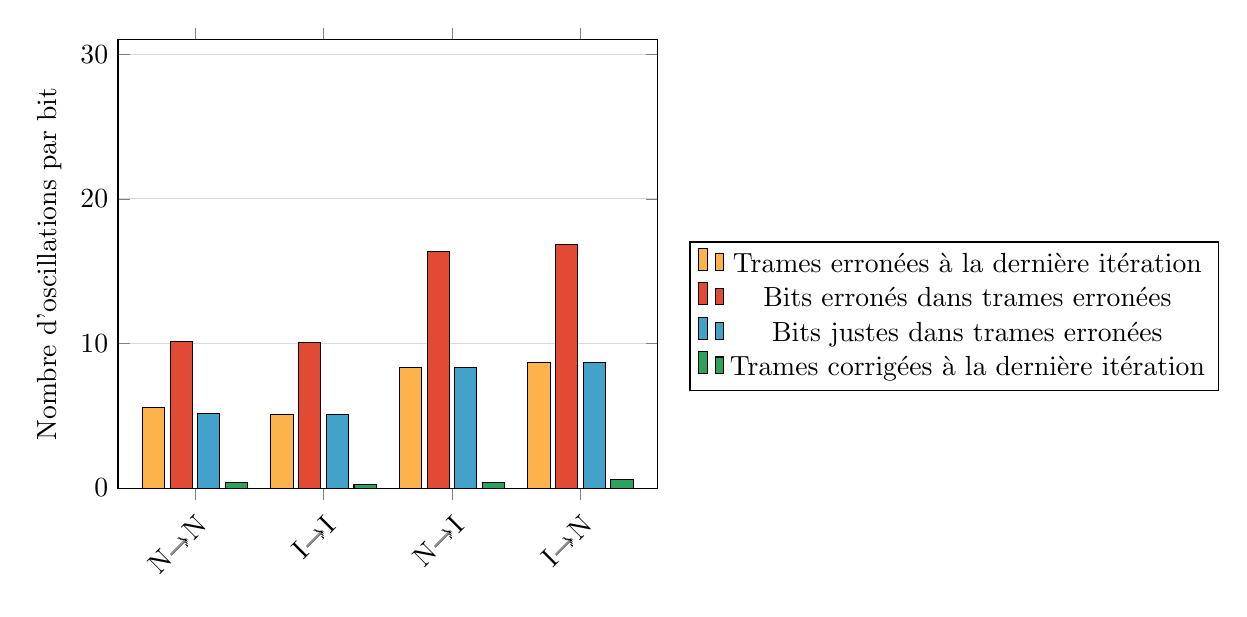
\begin{tikzpicture} 
    \begin{axis}[symbolic x coords={N\textrightarrow N, I\textrightarrow I, N\textrightarrow I, I\textrightarrow N},
                xtick=data,
                x tick label style= {rotate=45,anchor=north east},
                ylabel=Nombre d'oscillations par bit,
                ymin=0, ymax=31,
                legend style={at={(1.55,0.55)}, anchor=north, legend columns=1}, 
                ybar, bar width=8pt,
                enlarge x limits=0.2,
                ymajorgrids, grid style={gray!30},
                ] 

        \addplot[fill=falseframe] coordinates {(N\textrightarrow N,5.57395) (I\textrightarrow I,5.07164) (N\textrightarrow I,8.35103) (I\textrightarrow N, 8.6931)};
       
        \addplot[fill=falsebit] coordinates {(N\textrightarrow N,10.1565) (I\textrightarrow I,10.0708) (N\textrightarrow I,16.3818) (I\textrightarrow N,16.8692)};
        \addplot[fill=correctbit] coordinates {(N\textrightarrow N,5.17377) (I\textrightarrow I,5.07164) (N\textrightarrow I,8.35103) (I\textrightarrow N,8.6931)};

        \addplot[fill=correctframe] coordinates {(N\textrightarrow N,0.399922) (I\textrightarrow I,0.243594) (N\textrightarrow I,0.361816) (I\textrightarrow N,0.565654)};
        
        \legend{Trames erron\'ees \`a la derni\`ere it\'eration, Bits erron\'es dans trames erron\'ees, Bits justes dans trames erron\'ees, Trames corrig\'ees \`a la derni\`ere it\'eration} 


    \end{axis} 
\end{tikzpicture}
\end{document}